%====================================================================%
%                  MORIOND.TEX     2002                              %
% This latex file rewritten from various sources for use in the      %
% preparation of the standard proceedings Volume, latest version     %
% for the Neutrino'96 Helsinki conference proceedings                %
% by Susan Hezlet with acknowledgments to Lukas Nellen.              %
% Some changes are due to David Cassel.                              %
%====================================================================%

%\documentstyle[11pt,moriond,epsfig]{article}
\documentclass[11pt]{article}
\usepackage{moriond,epsfig}
%\usepackage{epsfig}
\usepackage{txfonts}
\usepackage{graphicx}
%%%%%%%%%%%%%%%%%%%%%%%%%%%%%%%%%%%%%%%%%%%%%%%%%%
%                                                %
%    BEGINNING OF TEXT                           %
%                                                %
%%%%%%%%%%%%%%%%%%%%%%%%%%%%%%%%%%%%%%%%%%%%%%%%%%
\begin{document}
\vspace*{4cm}
\title{Search for Optical Scintillation due to Interstellar Gas with LSST}

\author{Moniez, M.}

\address{Laboratoire de l'Acc\'{e}l\'{e}rateur Lin\'{e}aire,
{\sc IN2P3-CNRS}, Universit\'e de Paris-Sud, \\
B.P. 34, 91898 Orsay Cedex, France.
E-mail: moniez@lal.in2p3.fr}

\maketitle\abstracts{
}

\section{introduction}
Stars twinkle because their light propagates through turbulent atmosphere.
Of order of one percent light modulation due to scintillation
is expected to happen at a few minute time scale when remote stars are observed
through an interstellar turbulent cloud, but it has never been
observed at optical wavelengths.
The time scales of the weak optical intensity fluctuations resulting from the
wave distortions induced by a turbulent medium (visible nebulae or
hidden molecular gas) are accessible only now to the current technology.
LSST is the ideal setup to search for this signature of gas
thanks to the fast readout and to the wide and deep field.
As a first result, the detection of such a signal would provide a new tool to
measure the inhomogeneities and the dynamics of nebulae.
Our long term objective is to search for
{\it cold transparent} molecular $H_2$ {\it dust-free} clouds, which are the last possible
candidates for the missing baryons
%in cosmic structures on different scales
\cite{fractal}, \cite{pfre} representing $\sim 50\%$
of the Milky Way baryons \cite{mcetal}.
We propose to take long series of consecutive images of the same field
toward LMC or SMC during two nights through the "moving mode". This
"micro-survey" could be done during the commissioning of the camera,
but does not need all the mechanical functionalities of the telescope mount,
since the telescope should point at the same direction during the full nights.

\section{A new technique to search for the Galactic hidden baryons}
It has been suggested that a hierarchical structure of cold $\mathrm{H_2}$
could fill the Galactic thick disk\cite{fractal} or halo\cite{Jetzer1}, 
providing a solution for the Galactic dark matter problem.
This gas should form transparent (dust-free)
``clumpuscules'' of $10\,\mathrm{AU}$ size,
with a column density of $10^{24-25}\,\mathrm{cm^{-2}}$, and a
surface filling factor smaller than 1\%.
Such clumpuscules are invisible to the direct observations
since they do not emit or absorb light, but only increase the total optical path of the light by $5-50cm$;
as a consequence, the diffractive and refractive scintillation caused by their turbulence
- similarly to the well known radio scintillation - is the only way to detect them.

\begin{figure}[h]
\begin{center}
% \epsscale{0.8}
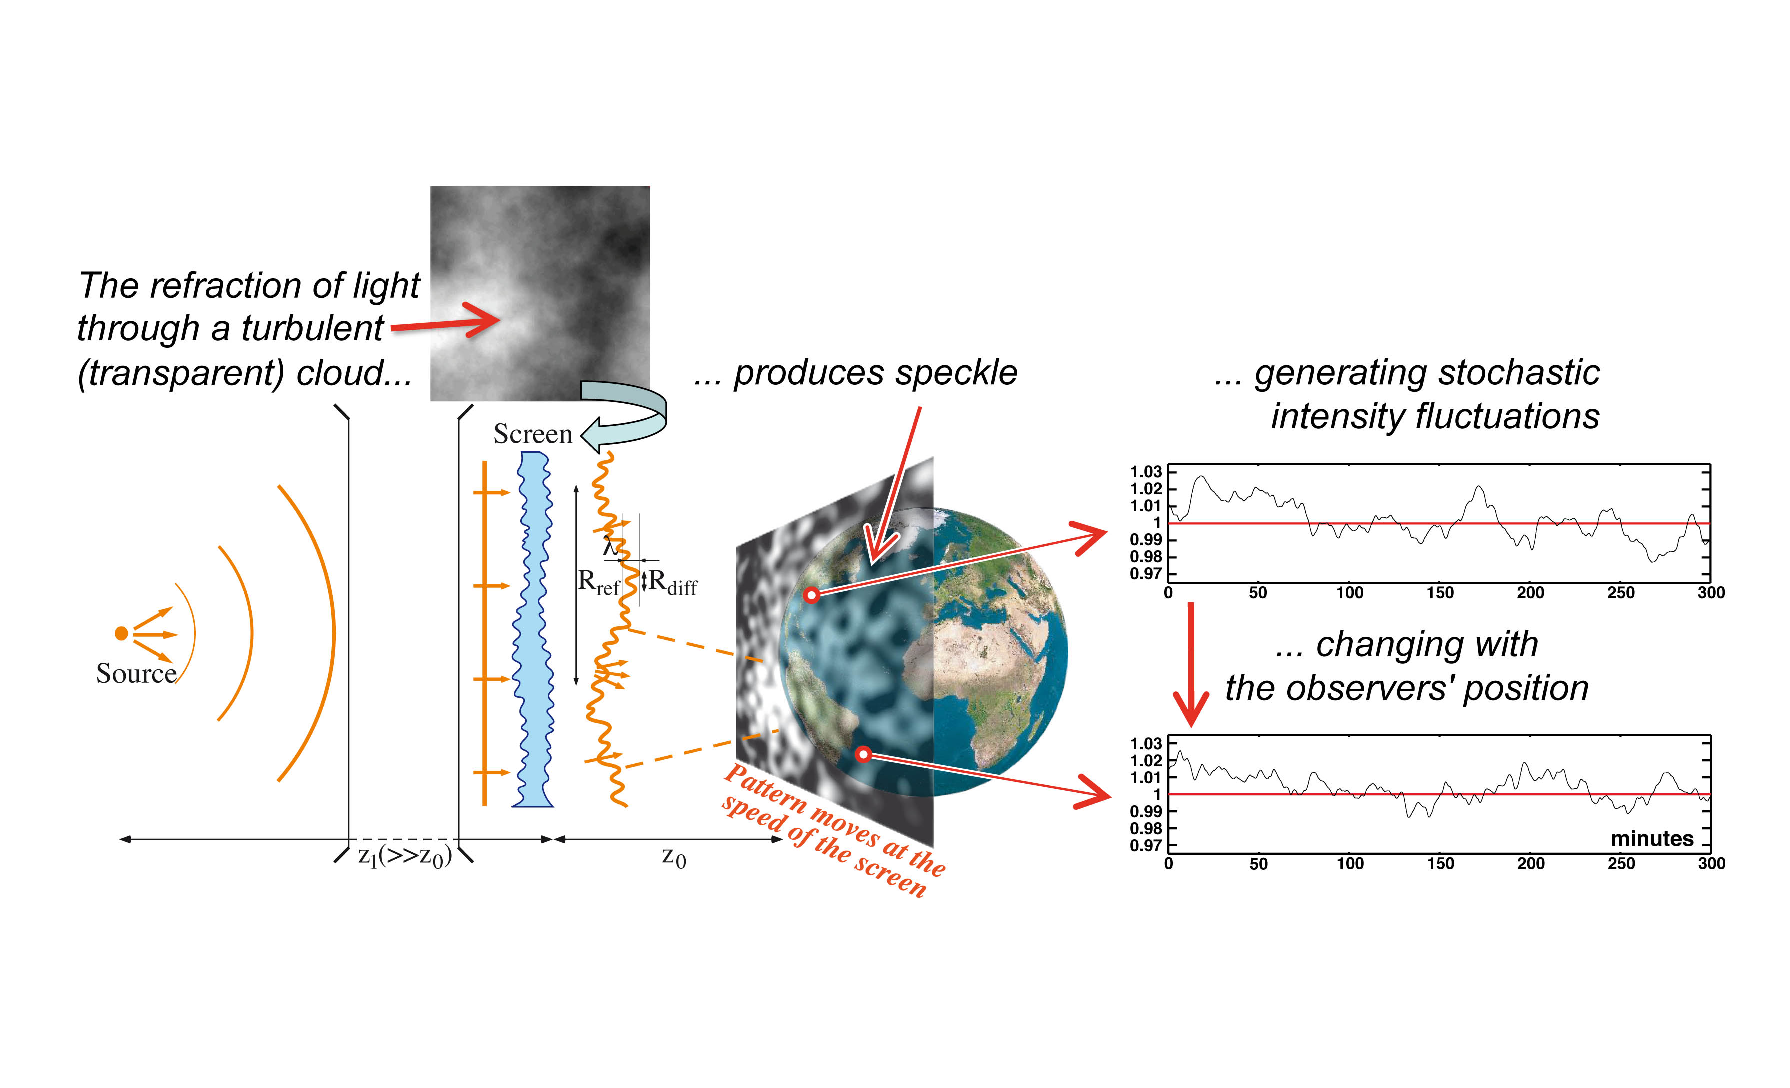
\includegraphics[angle=0,scale=.50]{principe_scintillation_2tels.pdf}
%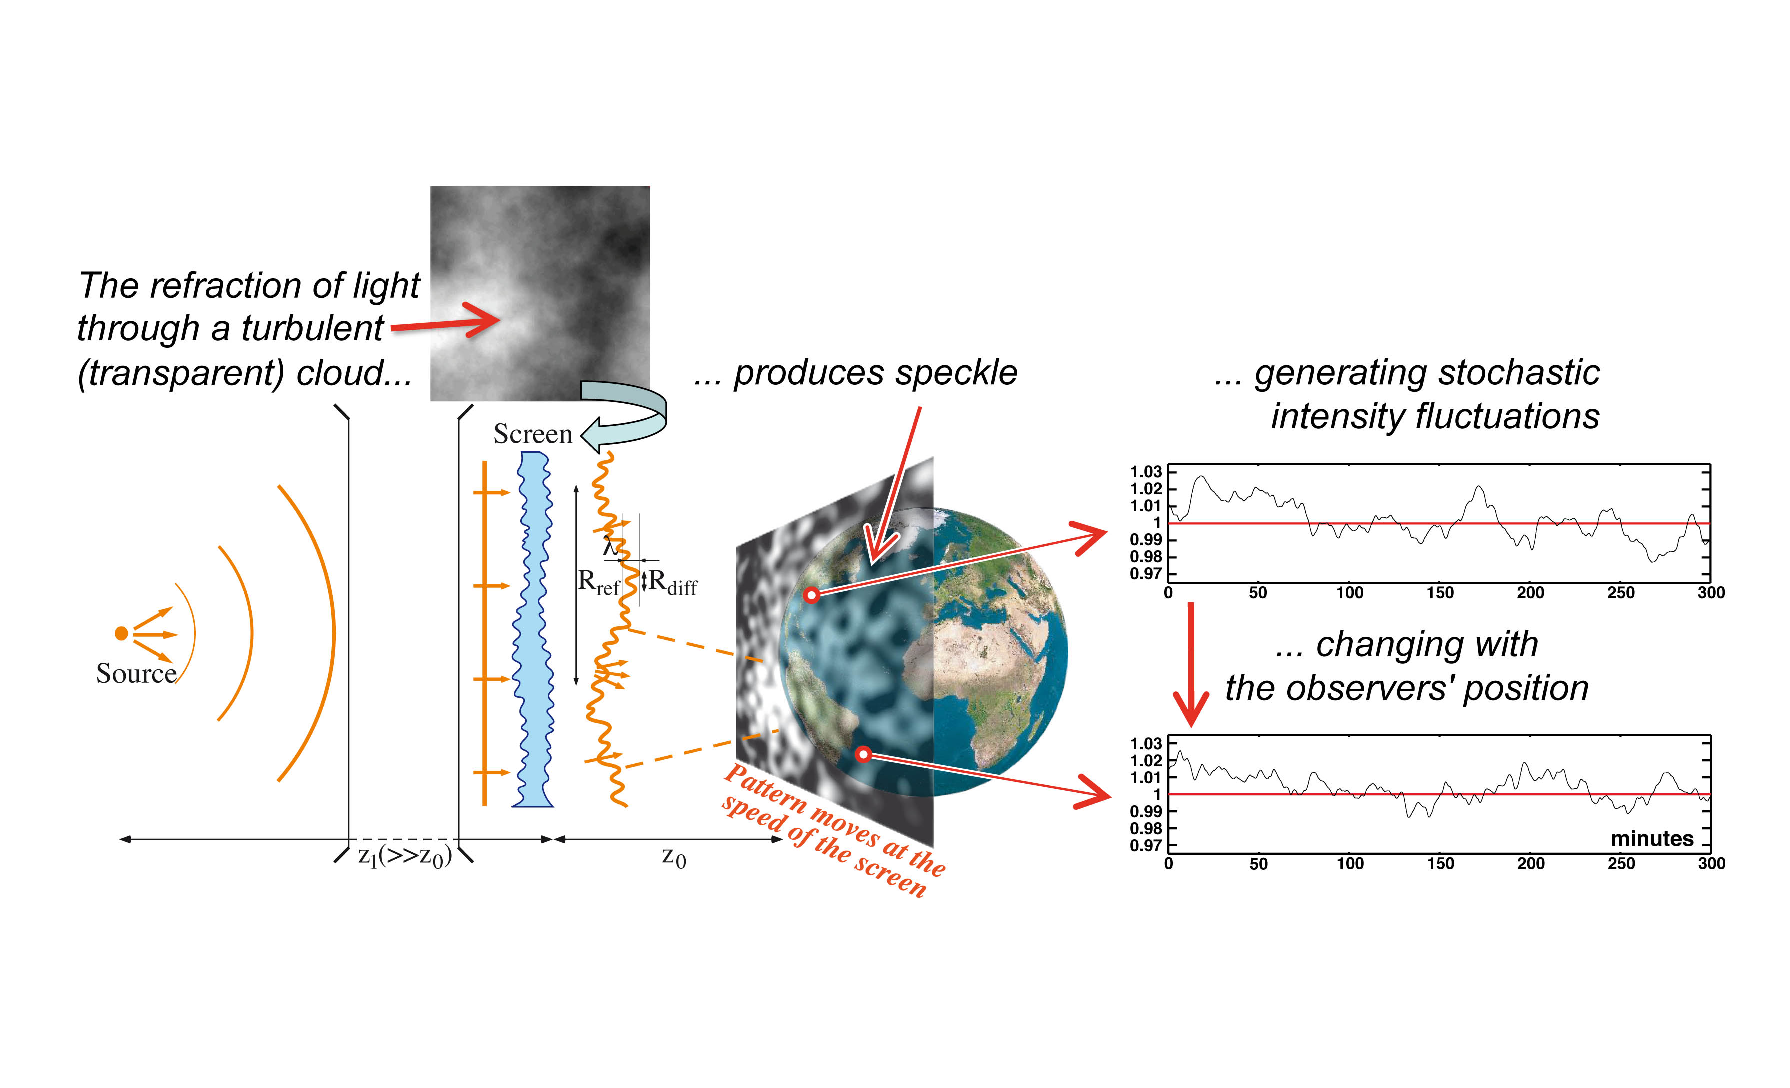
\includegraphics{principe_scintillation_2tels.pdf}
% \plotone{principe_scintillation_2tels.eps}
%\vspace{-2.5cm}
\end{center}
\caption
{\it
Up: simulation of a 2D stochastic phase delay (grey scale) caused by the
column of gas affected by Kolmogorov-type turbulence.
Down: the propagation of light from a stellar source (left)
after crossing the cloud (represented as a phase screen)
and the resulting illumination pattern
on Earth. The distorted wavefront produces structures at scale
$R_{ref}= 3086km\times
\left[\lambda/1\mu m \right]\left[z_0/100\,
    pc\right]\left[R_{diff}/1000\, km\right]^{-1}$.
As a consequence, two telescopes distant by a few thousand kilometers
are differently illuminated at a given time.
These structures sweep the Earth at the transverse speed
of the screen (typically a few $10\, 's$ of $km/s$), producing uncorrelated
illumination fluctuations at a few minute time scale.
The configuration simulated here corresponds to a scintillating star of half the solar size,
located at $1\, kpc$, seen through a turbulent cloud at $160\, pc$ with $R_{diff}=1000\, km$
translating at $V_T \sim 17\, km/s$ with respect to the line of sight. The two telescopes are
$10,000\, km$ away (the GEMINI telescopes are at $9430\, km$ linear distance).
}
\label{principe}
\end{figure}

Fig. \ref{principe} shows how refraction through an inhomogeneous transparent cloud
produces an irregular illumination on Earth (\cite{Moniez} and \cite{habibietal}).
The turbulence strength of the refractive medium is quantified by the
diffraction radius $R_{diff}(\lambda)$, defined as the transverse separation
for which the rms of the phase difference is 1 radian at $\lambda$.
The refractive medium, located at distance $z_0$ from Earth,
and moving with transverse velocity $V_T$
relative to the line of sight, is responsible for stochastic
intensity fluctuations of the light received from the star
at a typical {\bf characteristic time scale of a few minutes}, scaling as:
%\vspace{-0.5cm}
\begin{equation}
t_{ref}(\lambda) = %\frac{R_{ref}(\lambda)}{V_T} \sim
5.2\, minutes\left[\frac{\lambda}{1\mu m}\right]\left[\frac{z_0}{100\, pc}\right]\left[\frac{R_{diff}(\lambda)}{1000\, km}\right]^{-1}\left[\frac{V_T}{10\, km/s}\right]^{-1},
%\vspace{-0.2cm}
\label{dureescint}
\end{equation}
with a typical {\bf intensity modulation index $m_{scint.}=\sigma_I/<I>$ of a
few $\%$},
limited by the source spatial coherence, thus decreasing when
the angular stellar radius $\theta_r$ increases, according to:
%\vspace{-0.3cm}
\begin{equation}
m_{scint.} = 0.05 \, \left[\frac{\lambda}{1 \mu m}\right] \left[\frac{z_0}{100\, pc}\right]^{-1/6} 
                      \left[\frac{R_{diff}(\lambda)}{1000
                          km}\right]^{-5/6}
                      \left[\frac{\theta_r}{\theta(Sun\  at\  10 kpc)}\right]^{-7/6}.
%\vspace{-0.2cm}
\label{xparam}
\end{equation}
Since the illumination on Earth depends on the position (Fig. \ref{principe}-right),
we expect variations of the light-curves observed from two telescopes
to decorrelate when their distance increases. This signature
--  incompatible with an intrinsic source variability --
points to a propagation effect. \\
One should notice that the signal cannot be confused with atmospheric scintillation
- that induces fast PSF variations but negligible intensity variations within a large aperture \cite{dravins} - or with atmospheric absorption fluctuations, that can be precisely taken into account in the analysis, by the simultaneous monitoring of all stars in the field.

\section{Preliminary studies with the NTT and expectation with LSST}
A test has been performed on the NTT telescope, with the IR
SOFI detector through nebulae B68, cb131, Circinus and
towards SMC \cite{habibietal}. All sources of
background due to atmospheric effects, asterosismology, granularity of the
stellar surface, spots or eruptions
have been confirmed to be negligible at the few minutes time-scale variations.
One candidate to scintillation was found through nebula B68 within a sample
of $\sim 1100$ monitored stars (Fig. \ref{candidate}).
\begin{figure}[h!]
%\centering
\parbox{10.cm}{
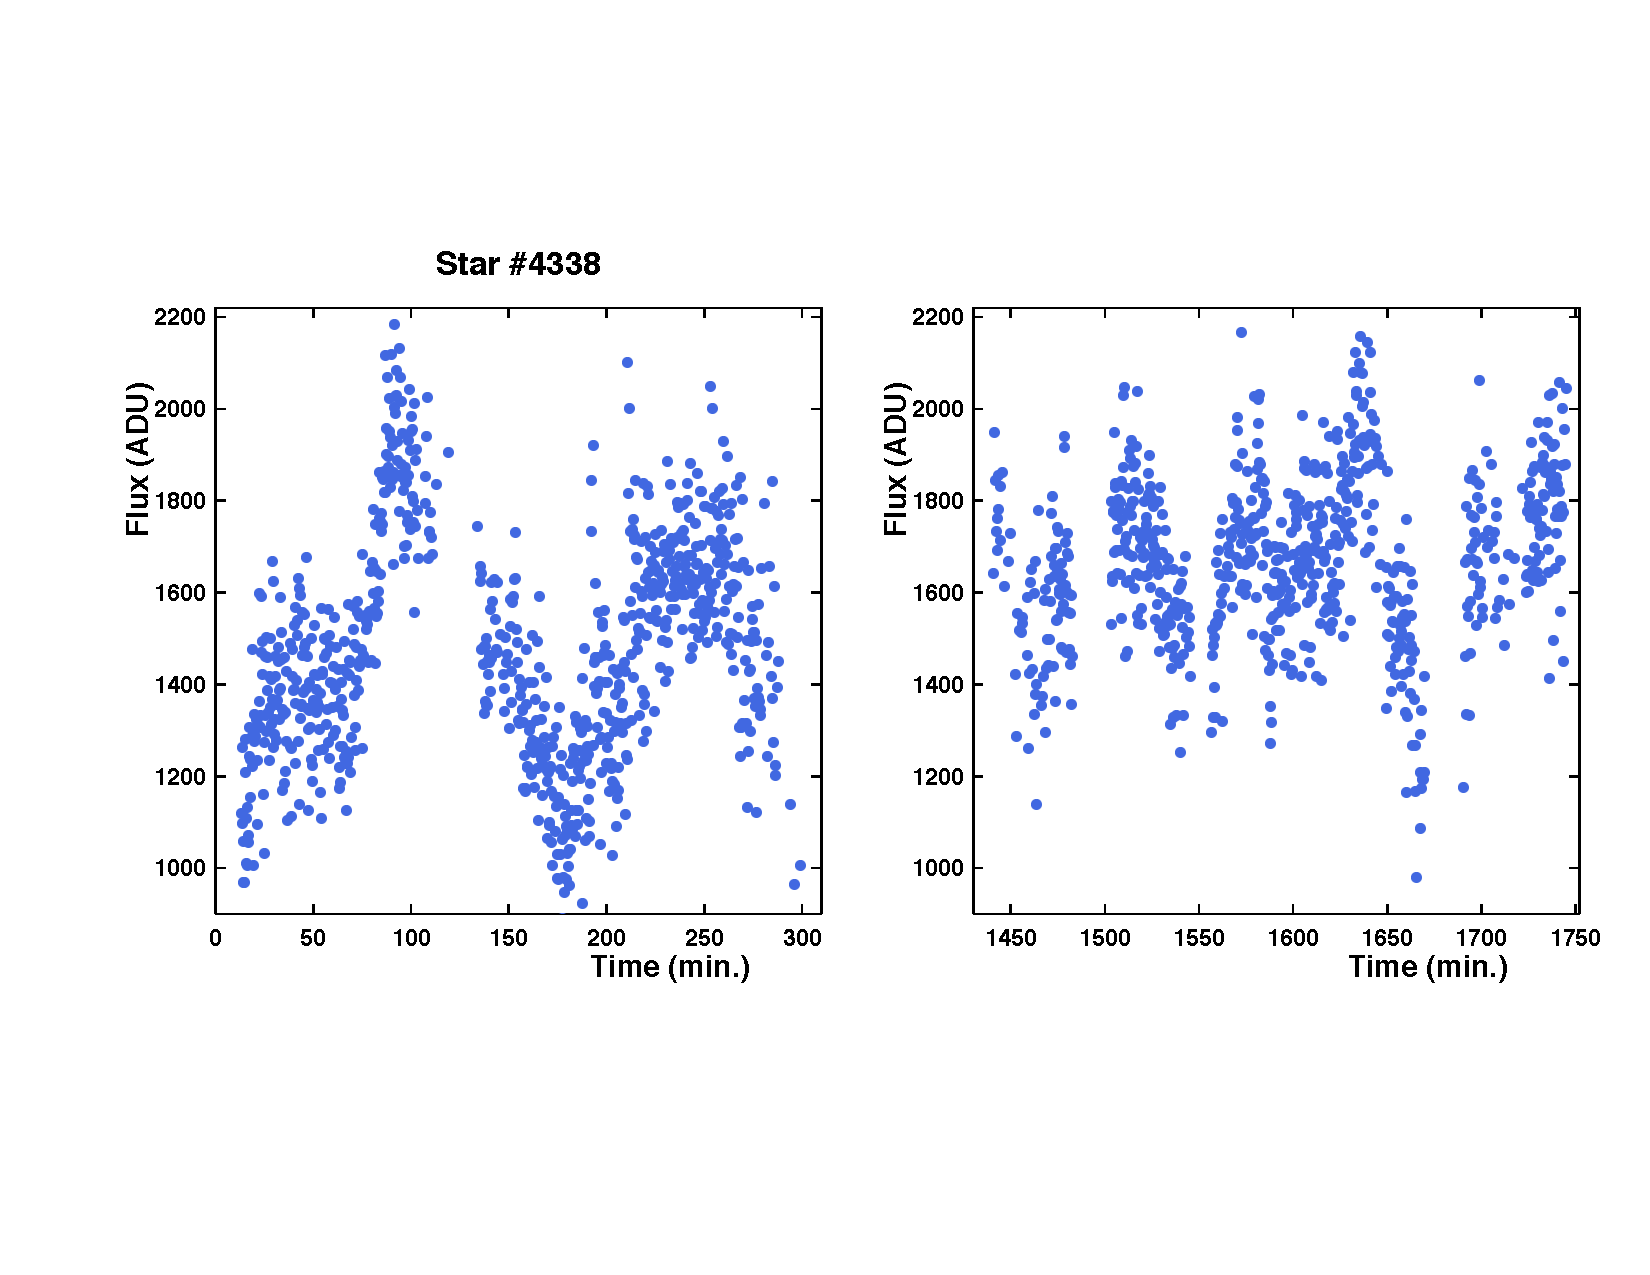
\includegraphics[width=10.cm]{15260fg11a.pdf}
%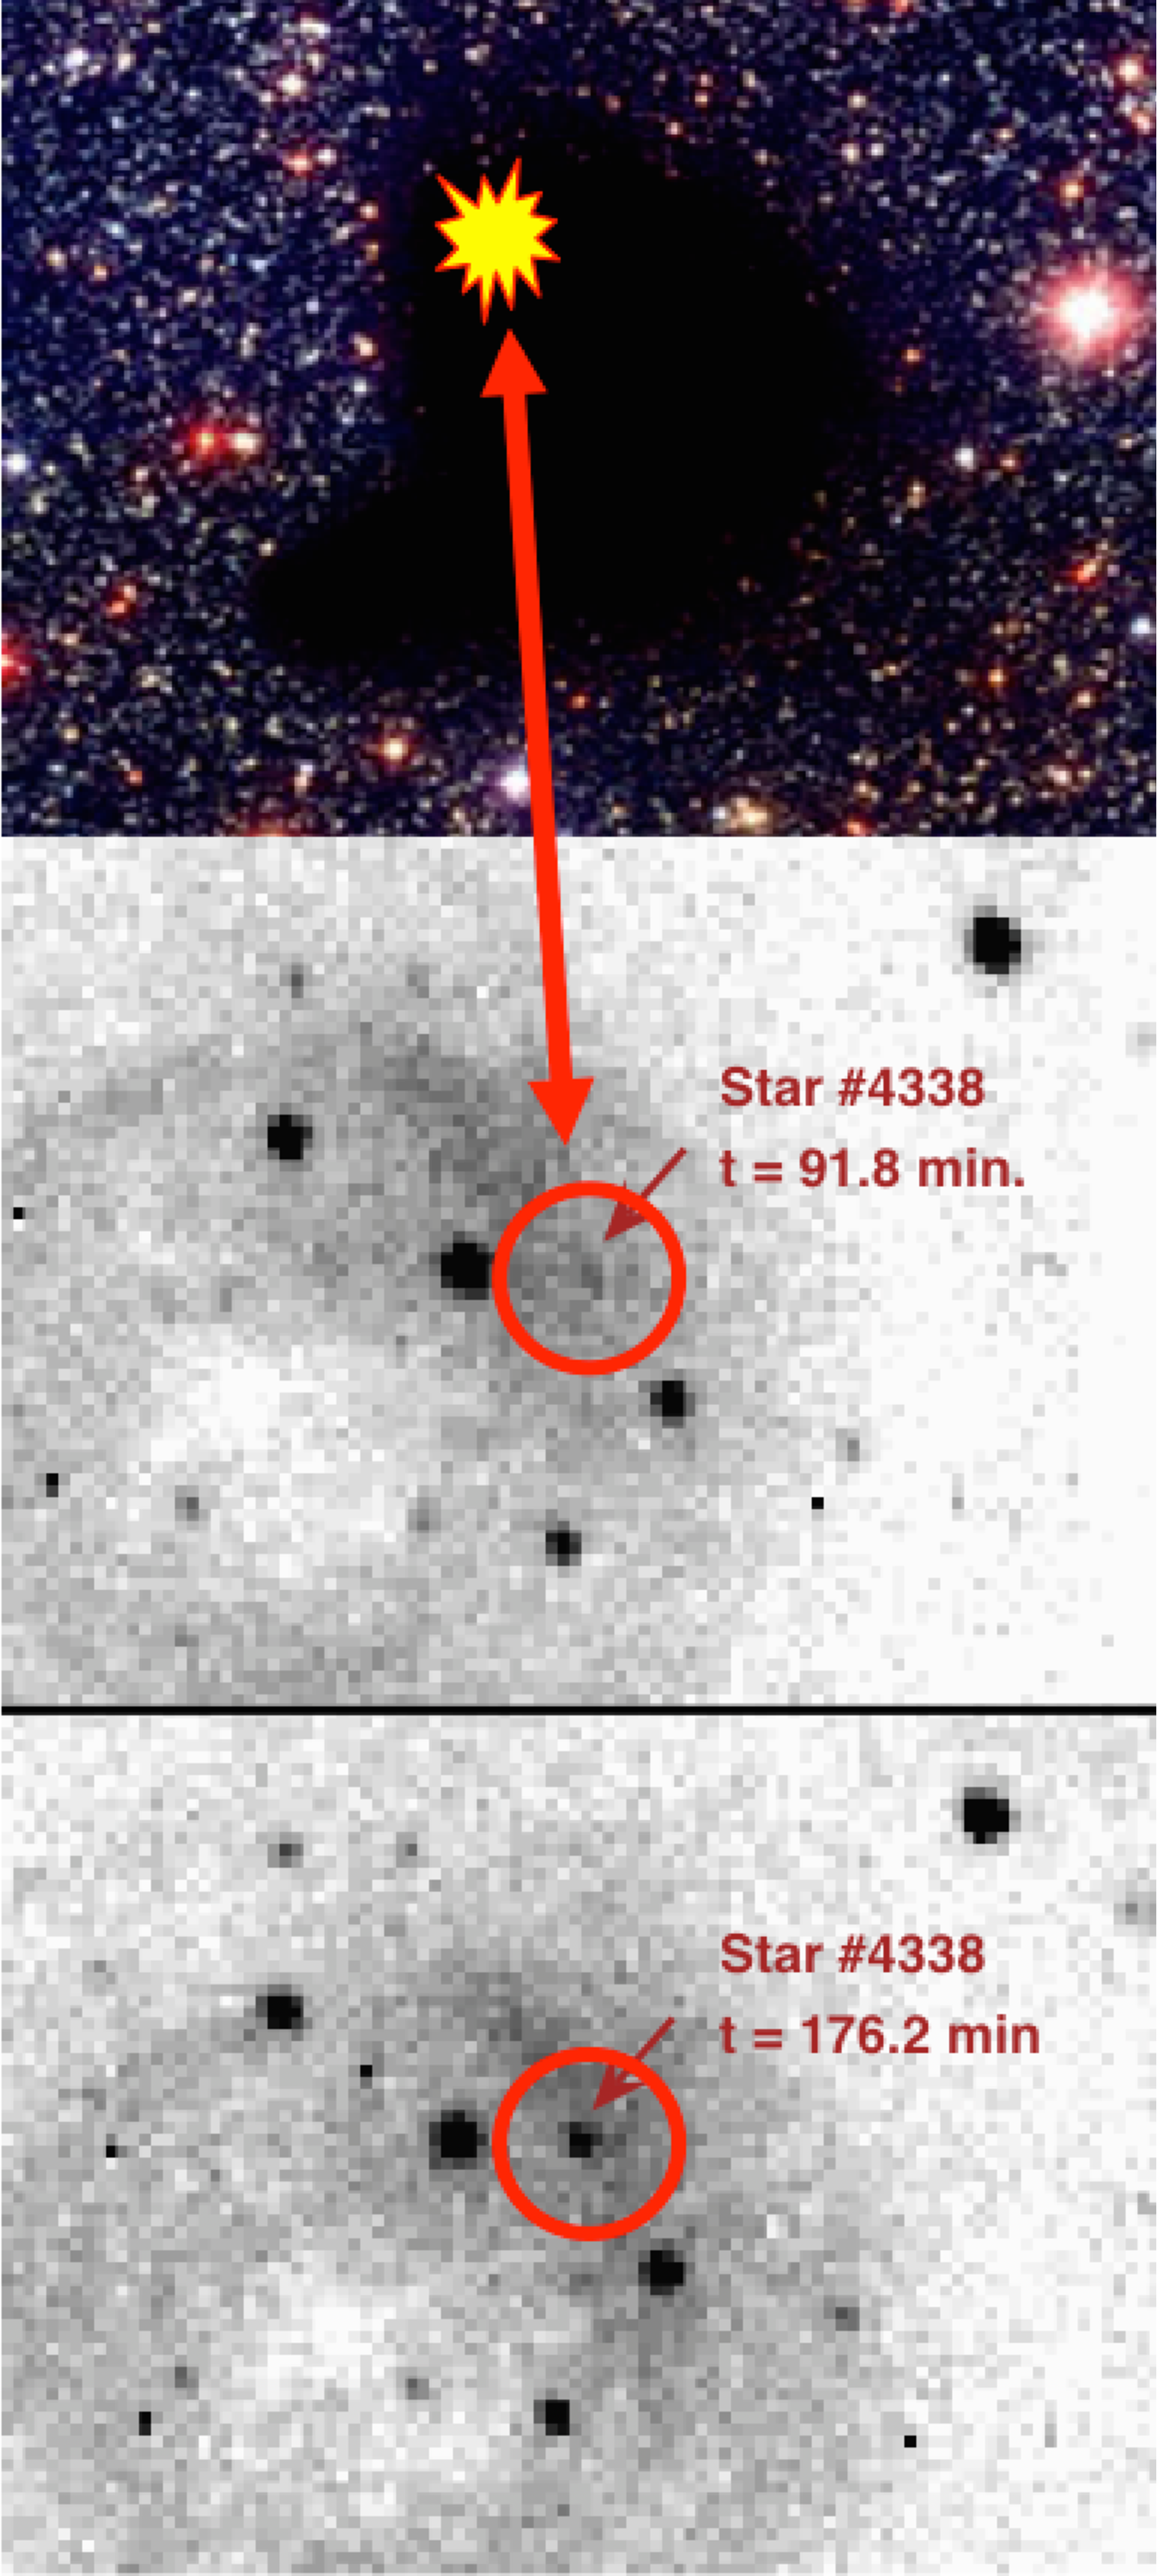
\includegraphics[width=5.5cm]{candidat-scint.pdf}
%\epsscale{0.5}
%\plotone{15260fg11a.eps}
\caption[]{\it
$K_S$ light-curves for the two nights of observation (above) and images of the
candidate ($<K_S>=16.6$, $<J>=20.4$) found behind B68 during a low-luminosity phase (middle-right)
and a high-luminosity phase (bottom); North is up, East is left.
These light-curves are compatible with scintillation produced by a very turbulent core with
$R_{diff}<100km$, corresponding to density fluctuations $\sigma > 1.5 \times 10^9 molecules/cm^{3}$.
The confirmation that scintillation is involved here would need simultaneous measurements from 2 distant places.
%The modulation index of the light-curve is $m=0.17$.
%\label{candidate}
}
}
%\hspace{0.3cm}
%\parbox{8.5cm}{
%\epsscale{0.25}
%\plotone{15260fg11b.eps}
%}
\hspace{0.3cm}
\parbox{5.7cm}{
%\includegraphics[width=5.5cm]{15260fg11b.pdf}
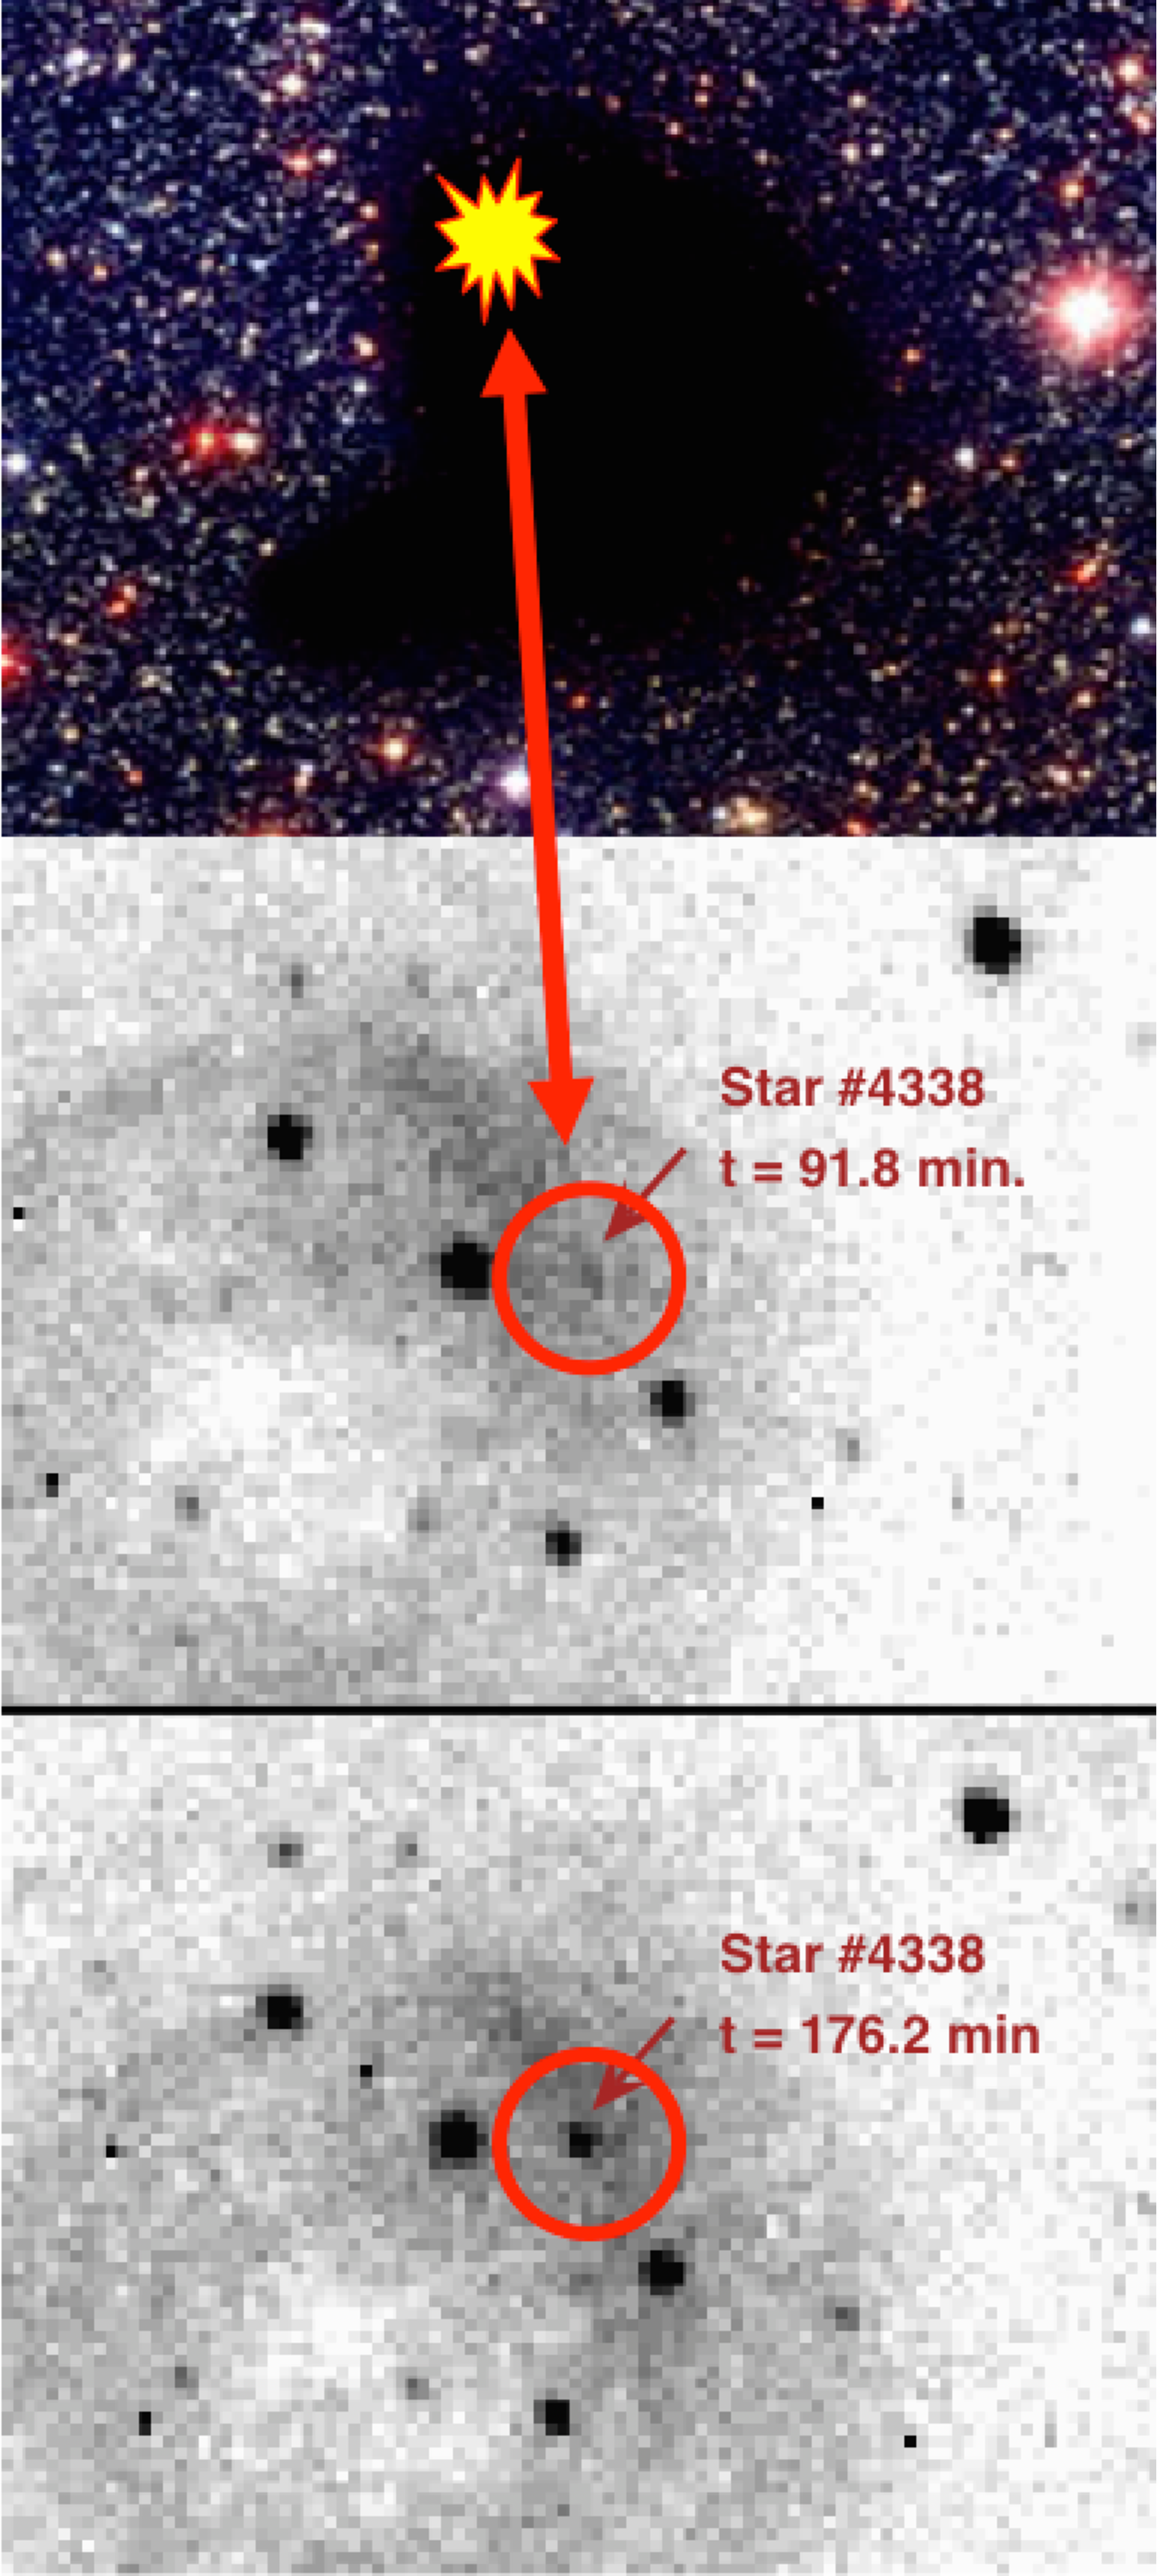
\includegraphics[width=5.5cm]{candidat-scint.pdf}
\label{candidate}
}
\end{figure}
An upper limit on the contribution of
invisible gaseous structures to the Milky-Way hidden mass % (Fig. 3).
has also been obtained from observations towards the SMC, thanks to a complete simulation of the process \cite{simul}.

Fig. \ref{expectations} shows the configurations (source magnitude and
turbulence strength expressed in $R_{diff}$) that should produce
detectable scintillation with LSST observations (upper-right zone).
The ultimate sensitivity corresponds to $R_{diff} \sim 16,000 km$, which is typically associated to a medium
with density fluctuations as low as $2\times 10^7\ cm^{-3}$.

\begin{figure}[h!]
\parbox{8.cm}{
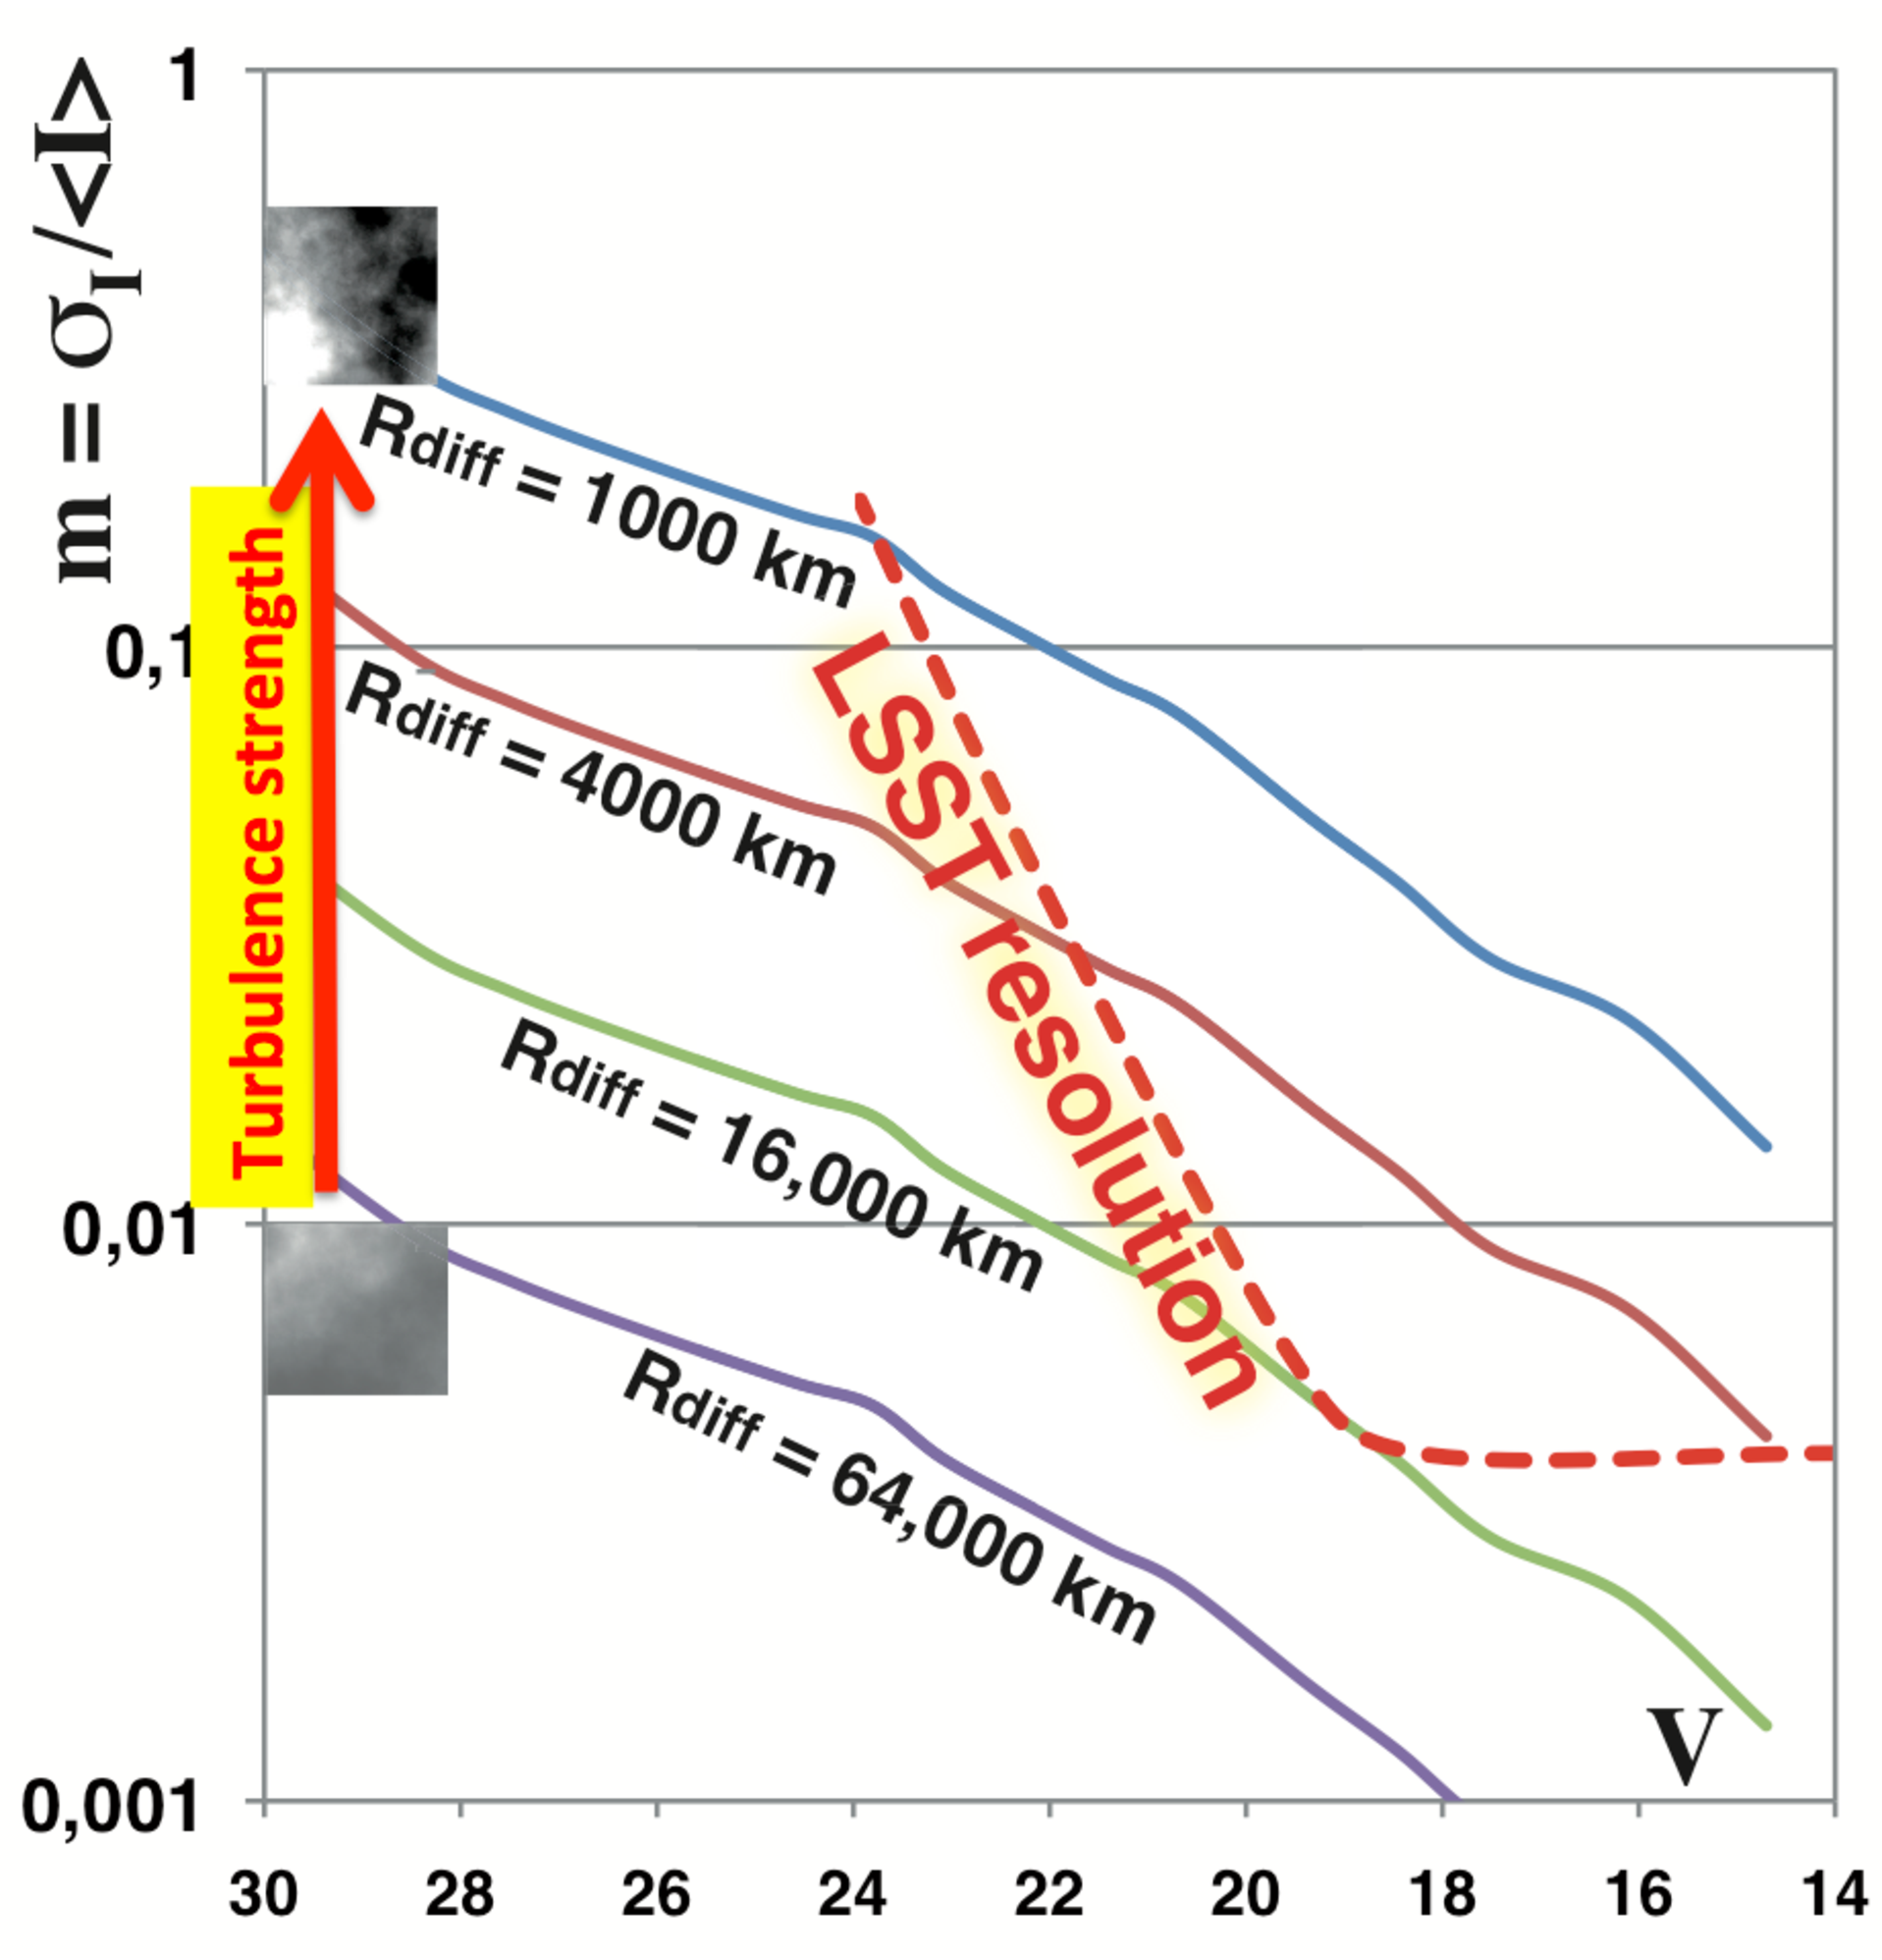
\includegraphics[angle=0,scale=0.25]{sensitivity-LSST.pdf}
}
\hspace{0.3cm}
\parbox{8.cm}{
\caption{ \it
The expected modulation index {\bf m} in $V$ , as a function of the source
apparent magnitude, for 4 different turbulence strength parameters $R_{diff}$ (smaller $R_{diff}$
corresponds to stronger turbulence).
The screen is at $z_0=1Kpc$ (invisible halo clumpuscule typical case), the source is at
$z_1=55Kpc$ (within LMC).
The instrumental photometric precision (dashed line) is taken from the LSST science book \cite{sciencebook}.
We see that few percent precision observations already allow a sensitivity to a
medium with relatively low strength turbulence, characterized by $R_{diff} < 16,000 km$,
that should induce scintillation detectable for stars with $16 < V < 22$. }
\label{expectations}
}
\end{figure}

\section{Strategy}
Using the LSST,
two runs (either with neutral filter, to benefit from a maximum of light, or
with g filter) of a few hours towards a given
direction (LMC or SMC to benefit from the wide field),
taking series of 15s consecutive exposures, will allow
to obtain a few tens of millions of light-curves with 1-2 thousands of measurements each
at the requested high rate ($\sim 3$ per minute) and the requested photometric
precision (better than 1\% on stars with $M_V=20.5$).
Such a harvest of data would allow to efficiently search for a scintillation signal down to
optical depth of order of $10^{-6}$.
\begin{itemize}
\item
If no scintillation is discovered, a strong upper limit of the molecular gas contribution
to the Galactic mass will be established (following the analysis of \cite{habibietal}).
\item
If a scintillation signal is suspected, it could be confirmed thanks to the repetition of the observations
during two different nights (which do not need to be consecutive).
Moreover, if a trigger is available at the time of observations (based on simple peak-to-peak variation
threshold), complementary observations could be simultaneously done with remote
telescopes, allowing to test the decorrelation of the stochastic fluctuations between
distant locations.
\item
If enough twinkling stars are discovered,
the decrease of the modulation index when the size of the source
increases could also be measured, as a check of the properties
of the scintillation process.
\end{itemize}

\section{Synergies}
The database produced by such a "movie mode" will certainly be useful for many other
science subjects like the searches for planetary transits, the detailed study of eclipsing
binaries (to refine the knowledge of the LMC distance), the microlensing
searches for hidden very low mass compact objects and for microlensing caustic crossing if
observations are coordinated with the microlensing networks.

\begin{thebibliography}{99}
\bibitem{habibietal}
Habibi, F., Ansari, R., Moniez, M. \& Rahvar, S., 2011, A\&A 525,
A108
\bibitem{dravins}
Dravins, D., Lindegren, L., Mezey, E., \& Young, A.T.,
Pub. of the Ast. Soc. of the Pacific, 1997,
109 (parts I and II), 1998, 110 (part III)
\bibitem{simul}
Habibi, F., Moniez, M., Ansari, R., \& Rahvar, S., 2013, A\&A 552, A93
\bibitem{mcetal}
McGaugh et al., M. J. ApJ, 708: L14-L17, 2010
\bibitem{Moniez}
Moniez, M., 2003, A\&A 412, 105
\bibitem{fractal}
Pfenniger, D., \& Combes, F. 1994, A\&A, 285, 94
\bibitem{pfre} 
Pfenniger, D., Revaz, y. A\&A 431,511-516 2005
\bibitem{sciencebook}
LSST Science Collaborations and LSST Project 2009, LSST Science Book,
Version 2.0, arXiv:0912.0201
\end{thebibliography}
\end{document}
